\addchap{Preface}

This document is not a beginner guide.
There is a wide choice of those out there already, both free and paid for.
However, what is lacking is a collection of modern, or even at least current,
best practices.
If you scouted through package documentations and
\href{https://tex.stackexchange.com/}{StackExchange}
long enough, you would eventually get an idea of what is current, idiomatic \LaTeX{}
and what is not.
This is how I learned \LaTeX{} too, so I cannot recommend any useful beginner books.
You might want to check out \href{https://www.overleaf.com/}{Overleaf} though,
an online \LaTeX{} editor%
\footnote{%
    I do not recommend using online editors.
    You are putting your hard work onto some remote, foreign server, relying on
    their ongoing availability and forfeiting the chance of understanding \LaTeX{},
    in case you have to continue locally.
    Theses containing confidential material should also not be hosted externally.
}
with a large knowledge database.

This document is an attempt at collecting best practices
--- or at least, useful approaches ---
and pointing out the old ones they could, and often should, replace.
More than most other languages, the \LaTeX{} code in circulation world\-/wide is
quite aged.
While that code does not necessarily get \emph{worse}, it also does not exactly
age like cheese and wine would.
To that end, notice how the packages integral to this document are actively
maintained and kept modern.

\paragraph{Usage as a Cookbook}
This document is supposed to be used in a \emph{cookbook} style.
That is, it is not meant to be read cover to cover
(declaring it a cookbook is also a useful excuse for the mess I made).

The document contains various \enquote{recipes}, most of which exist in parallel and
are independent of one another.
The goal is to answer questions of the form \emph{How can this and that be done?}
A quick search in the (printed) output or the source code is supposed to deliver
answers.

\paragraph{Usage as a Template}
Considerable effort went into the class file, aka the template.
It pulls all settings together, producing an output that is very different from
vanilla \LaTeX{}.
Therefore, feel free to rip out all the cookbook content, keeping just the settings
files to be used as a template.

\paragraph{Source Code}
This document is meant to be read side\-/by\-/side with its source code.
That is why there is almost no source code in the printed output itself.
If you are curious how a certain output is achieved, navigate to the source code
itself.
This approach was chosen since, plainly, code does not lie, while annotations and
comments might.
So while the printed output will always remain true to its actual source code,
duplicating that source code so it can be read in the printed output directly
is just another vector for errors to creep in.

\section*{Beginning Prerequisites}

Since this document will probably still be read by people new to \LaTeX{}, there
will be a short description on how to get started below.
\LaTeX{} requires three things:
\begin{enumerate}
    \item of course, a source text file, ending in \texttt{.tex}.
        A minimal example is:

        \begin{lstlisting}[
            style=betweenpar,
            language={[LaTeX]TeX},
        ]
            \documentclass{scrartcl}
            \begin{document}
                Hello World!
            \end{document}
        \end{lstlisting}
        Note the usage of \texttt{scrartcl} over the standard \texttt{article}.
        This is a \ctanpackage{koma-script} document class.
        There are only \href{https://tex.stackexchange.com/a/73146/120853}{two reasons}
        why you would not use that package, both of which usually do not apply.
        \ctanpackage{koma-script} replaces the conventional \texttt{documentclass}
        like so:

        \begin{tabular}{
            @{}
            l
            @{ \textrightarrow{} }
            l
            @{}
        }
            \texttt{article} & \texttt{scrartcl} \\
            \texttt{report} & \texttt{scrreprt} \\
            \texttt{book} & \texttt{scrbook}
        \end{tabular}

        There is also a \texttt{letter} class, making writing formal letters a walk
        in the park.
        \ctanpackage{komascript} will provide you with a very large host of tools
        and settings that work very well indeed.
        Those combine most options you would otherwise get from other packages into
        one convenient class.
        Included are, among others:
        \begin{itemize}
            \item \ctanpackage{scrlayer-scrpage} instead of \ctanpackage{fancyhdr} for
                page styles, headers, footers \iecfeg{etc.},
            \item \ctanpackage{tocbasic} to modify the Table of Contents and other lists,
                and
            \item \ctanpackage{scrlttr2} for typesetting letters.
        \end{itemize}
        If the document loads a \ctanpackage{koma-script} document class, these
        packages are already available.
        However, the \ctanpackage{koma-script} defaults are also great
        (like using \texttt{a4paper} over \texttt{legal}),
        so you can also get started without dealing with options or packages at all.
        Just use it everywhere and profit.
        A viable alternative is \ctanpackage{memoir}, though I never used that.
    \item a \emph{distribution}, which are the compilers, packages and other
        goodies like fonts:
        \begin{itemize}
            \item \emph{Compilers} translate high\-/level source code (see the
                first point) to a different \enquote{language}.
                In our case, the other language is \abb{portable_document_format}
                source code.
                It is not human\-/readable and mostly gibberish, but a
                \abb{portable_document_format} viewer takes care of that.
            \item \emph{Packages} are bundles of ready\-/made functionalities for
                \LaTeX{}.
                There are packages for basically everything.
                The \href{https://ctan.org/}{\abb{comprehensive_tex_archive_network}},
                a \emph{package repository}, contains basically all of them.
        \end{itemize}
       UNIX-based operating systems do well with
       \href{https://www.tug.org/texlive/}{TeXLive},
       which is available as a package for most distributions.
       It is also available for Windows.
       It has a yearly release schedule.
       So there might be \href{https://tex.stackexchange.com/a/476742/120853}{bugs}
       that do not get fixed for a whole while.
       Nevertheless, I can recommend it.

       Another viable alternative is \href{https://miktex.org/}{MiKTeX}.
       It has a rolling release model, aka updates to packages are published
       whenever they are deemed ready.
       MiKTeX's \abb{graphical_user_interface} (the \emph{MiKTeX Console}) is pretty
       polished and usable, see \cref{fig:miktex_gui}.

       \begin{figure}
            \ffigbox[\FBwidth]{%
                \caption[%
                    % Do not use regular glossaries-commands in captions (or
                    % section headers etc.): if they occur in the LoC/LoT etc.,
                    % they will be expanded there already, which is unwanted.
                    MiKTeX \glsfmtlong{abb.graphical_user_interface} on Windows%
                ]{%
                    MiKTeX \abb{graphical_user_interface} on Windows%
                }%
                \label{fig:miktex_gui}%
            }{%
                % Having issued \graphicspath globally, we do not have to specify
                % the full path here. Not even a file extension is necessary.
                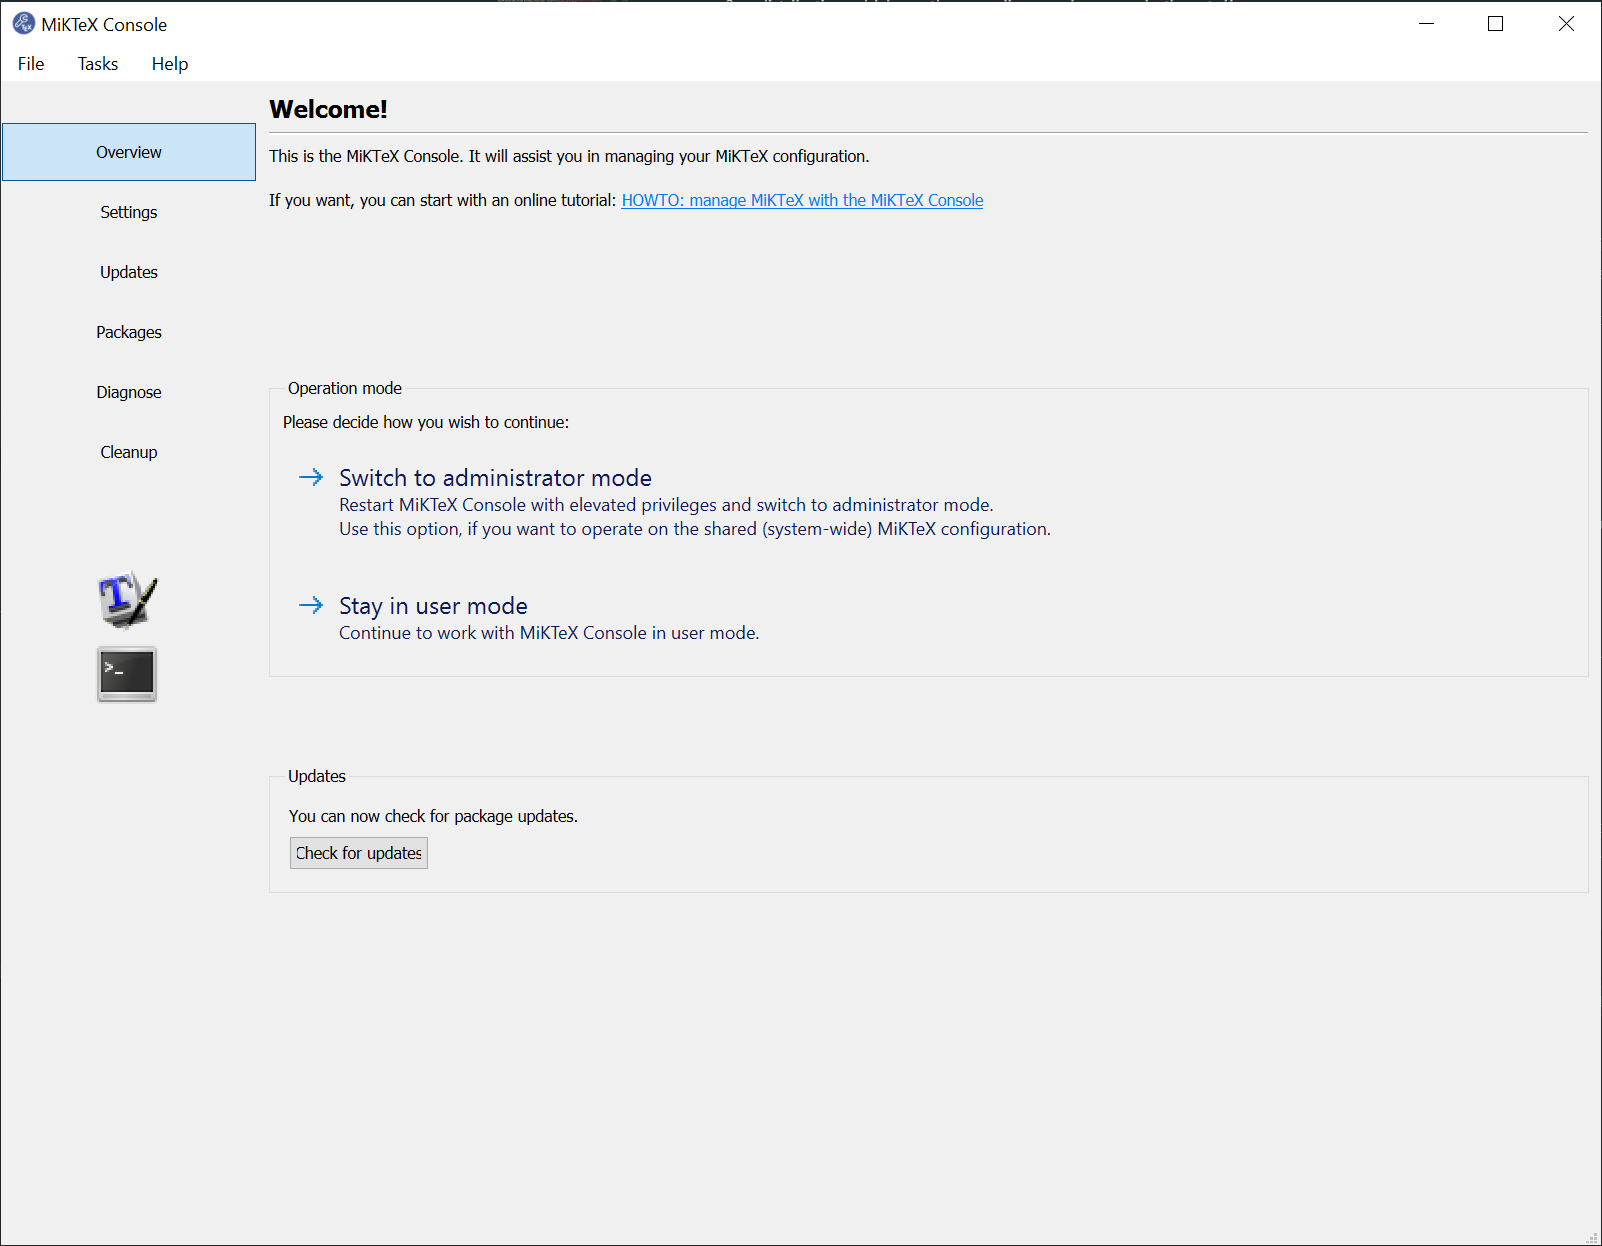
\includegraphics[width=0.8\textwidth]{miktex_gui}
            }
       \end{figure}

       You should hit that juicy \emph{Check for updates} at least yearly, rather
       biannually.
       \LaTeX{} is a slow world, in which files from the previous millennium might
       very well still compile and look fine.
       However, a very large share of errors are caused by out\-/of\-/date packages.
       For example, if your \LaTeX{} distribution is ancient (anything older than,
       say, three years), and you then compile a new file that installs a new
       package, you suddenly have that package in its latest version, alongside
       all the old packages.
       That will not go well long.
    \item of course, an \emph{editor}.

       Here, you are free to do whatever you want.
       I recommend \href{https://code.visualstudio.com/}{Visual Studio Code}, using its
       \href{https://marketplace.visualstudio.com/items?itemName=James-Yu.latex-workshop}%
       {\LaTeX{} Workshop} extension, which provides syntax highlighting, shortcuts
       and many other useful things.
       VSCode is among the most state\-/of\-/the\-/art editors currently available.
       Being usable for \LaTeX{} is just a nice \enquote{side\-/effect} we can take
       advantage of.

       For a more conventional, complete \abb{integrated_development_environment},
       try \href{https://www.texstudio.org/}{TeXStudio}.
       Like VSCode, it is also
       \href{https://github.com/texstudio-org/texstudio}{open source}.
       TeXStudio will cater to \SI{99}{\percent} of your \LaTeX{} needs.

       If you like to live dangerously, you can even write your \LaTeX{} in Notepad.
        Vim is not mentioned here because its users will probably have skipped this
        section\dots{}
\end{enumerate}

\subsection*{Compiling this document}

This document leverages many more advanced and demanding packages.
In this context, \emph{demanding} means that they sometimes need outside tools,
since \hologo{LuaLaTeX} aka plain \TeX{} were insufficient for their implementation.
This is most prevalent in packages that need sorting functionalities.
Therefore, compiling this document is a bit more involved than a simple call to
\texttt{pdflatex}.
To make it work for everyone, a Docker container is made available.
It includes all the tools required.
For more info, see the
\href{https://collaborating.tuhh.de/cap7863/latex-git-cookbook/-/blob/master/README.md}{README}
for the repository.

Outside tools are required for
\begin{enumerate}
    \item \ctanpackage{glossaries-extra}: requires the outside tool
        \ctanpackage{bib2gls}, see \cref{ch:bib2gls}.
    \item \ctanpackage{biblatex}: requires the outside tool \ctanpackage{biber},
        see \cref{ch:bibliography}.
\end{enumerate}
If you have a proper \LaTeX{} distribution, \texttt{bib2gls} and \texttt{biber}
will already be available as commands.
However, for everything to work, the following has to be installed:
\begin{itemize}
    \item \texttt{bib2gls} requires a Java Runtime Environment, which is
        \href{https://www.java.com/en/download/}{freely available for personal use},
    \item the \ctanpackage{svg} package requires the outside program
        \href{https://inkscape.org/}{InkScape}, which also has to be on your
        \texttt{\$PATH},
    \item using \texttt{contour gnuplot} commands with \ctanpackage{pgfplots} requires
        \href{http://www.gnuplot.info/download.html}{gnuplot} to be on the \texttt{\$PATH}.
\end{itemize}

To compile the entire document from scratch, install these things manually.
To never worry about installing and keeping things in order manually, use the provided
Docker container.

\paragraph{Compilation}
With the prerequisites done, the compilation itself can start.
For it, call:
\begin{enumerate}
    \item \texttt{lualatex}
    \item \texttt{biber}
    \item \texttt{bib2gls}
    \item \texttt{lualatex}
    \item \texttt{lualatex}
\end{enumerate}
This should get all the references right, set up the bibliography and the glossaries,
which in turn fills out any missing (\texttt{??}) entries.
I say \emph{should} because I never ran through this chain myself.
Instead, there is the \texttt{latexmk} tool to ease all this painful labour.
\texttt{latexmk} automates \LaTeX{} compilation by detecting all the required
steps and then running them as often as required.
It requires Perl.
Linux users will already have it available, Windows users may grab
\href{http://strawberryperl.com/}{Strawberry Perl}.

Once that is done, the entire document can be compiled by simply calling
\texttt{latexmk}.
You do not even have to provide a \texttt{*.tex} file argument.
By default, \texttt{latexmk} will simply compile all found \texttt{*.tex} files.
The core ingredient to this magic process is the \texttt{.latexmkrc} configuration file.
You can find it in the repository root directory.
It is tailored to this document and does not need to be touched if the compilation
process itself has not changed.
It also contains some more insights to the entire process.

\texttt{latexmk} is great because it figures out most things by itself and enjoys
wide\-/spread acceptance and adoption.
As such, chances are your \LaTeX{} editor either supports or outright relies on it
already.

Having walked through all this manually, hopefully using the prepared Docker image
instead makes more sense now.
Taking a look at \texttt{.gitlab-ci.yml} in the project root, we can see how easy it
can be:
run Docker container, call \texttt{latexmk}.
That is it!
It is guaranteed to work for everyone, because the Docker container (that is, the
virtual machine) will be identical for all users.
It is independent of local \LaTeX{} installations and all their quirks.
It will continue to work forever (the underlying software versions are fixed) and the
generated output will be identical for everyone.

If all of this is embedded into a pipeline on GitLab, your documents are built whenever
you \texttt{git push} to the remote server.
It does not get simpler; the downside is of course the lengthier setup, but all of that
is explained in the
\href{https://collaborating.tuhh.de/cap7863/latex-git-cookbook/-/blob/master/README.md}{README}.
Also, the repository itself is a live demonstration!
